% !TEX TS-program = LuaLaTeX-shell

\documentclass[convert,tikz,border=5pt]{standalone}
\usepackage{tikz}
\usetikzlibrary{positioning}
\tikzset{my node/.style={draw,thick,font=\sffamily, align=center,text width=3cm,minimum height=2cm,rounded corners,fill=#1}}
\begin{document}
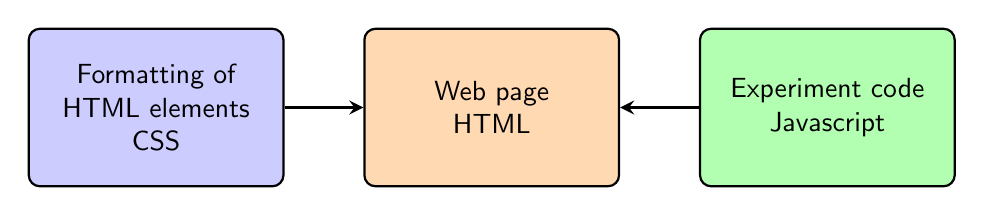
\begin{tikzpicture}
\node[my node=orange!30] (A) {Web page\\HTML};
\node[my node=blue!20] (B) [left=1cm of A] {Formatting of HTML elements\\CSS};
\node[my node=green!30] (C) [right=1cm of A] {Experiment code\\Javascript};
\draw[-stealth,very thick] (B) -- (A);
\draw[-stealth,very thick] (C) -- (A);
\end{tikzpicture}
\end{document}